\documentclass{article}%
\usepackage[T1]{fontenc}%
\usepackage[utf8]{inputenc}%
\usepackage{lmodern}%
\usepackage{textcomp}%
\usepackage{lastpage}%
\usepackage[head=40pt,margin=0.5in,bottom=0.6in]{geometry}%
\usepackage{graphicx}%
%
\title{\textbf{Secuela de "Suicide Squad" se quedó sin Will Smith}}%
\author{Diario El Universal}%
\date{04/03/2019}%
%
\begin{document}%
\normalsize%
\maketitle%
\textbf{URL: }%
http://www.eluniversal.com/entretenimiento/34703/secuela{-}de{-}suicide{-}squad{-}se{-}quedo{-}sin{-}will{-}smith\newline%
%
\textbf{Periodico: }%
EU, %
ID: %
34703, %
Seccion: %
entretenimiento\newline%
%
\textbf{Palabras Claves: }%
NO\_TIENE\newline%
%
\textbf{Derecho: }%
2.1%
, Otros Derechos: %
\newline%
%
\textbf{\textit{El popular actor, uno de los mejor pagados de Hollywood, no pudo cuadrar su agenda de compromisos con el rodaje de la cinta de acción}}%
\newline%
\newline%
%
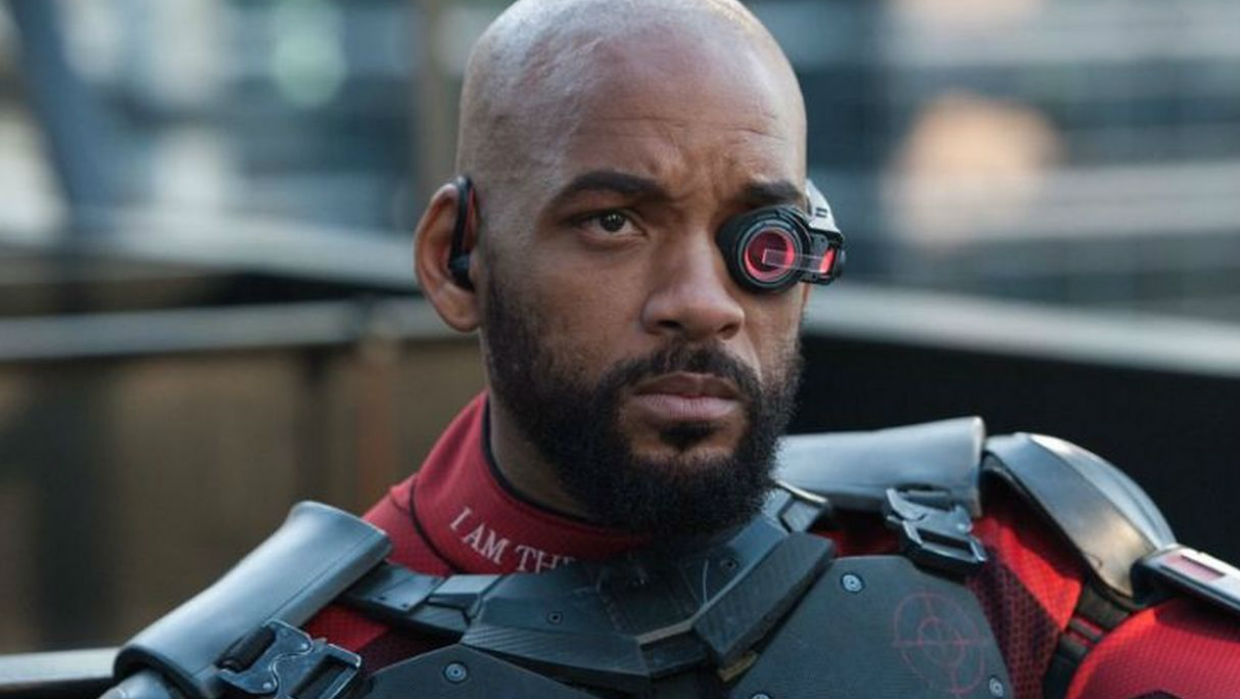
\includegraphics[width=300px]{EU_34703.jpg}%
\newline%
%
Los Ángeles.{-} Will Smith, uno de los protagonistas de la cinta de acción%
\newline%
%
(2016), no actuará en la secuela de esta cinta de antihéroes de Warner Bros. que dirigirá James Gunn, informó la revista%
\newline%
%
.%
\newline%
%
La imposibilidad de ajustar la agenda del actor parece estar detrás de su renuncia a interpretar nuevamente al personaje de Deadshot.%
\newline%
%
Smith estrenará en mayo la nueva versión de Aladdin, de la factoría Disney, y en 2020 estrenará Bad Boys for Life, tercera entrega de la saga de comedia y acción Bad Boys que protagoniza junto a Martin Lawrence.%
\newline%
%
La secuela de Suicide Squad, que se estrenará en agosto de 2021, no será una continuación sino una nueva mirada a este mundo de antihéroes con un reparto nuevo en su mayoría.%
\newline%
%
La primera entrega tuvo como protagonistas a Will Smith, Margot Robbie y Jared Leto bajo la dirección de David Ayer, y recaudó 746 millones de dólares, pero tuvo una fría recepción por parte de la crítica.%
\newline%
%
El fichaje de Gunn fue muy comentado en Hollywood puesto que tuvo lugar poco después de que fuera despedido por Disney como director de Guardianes de la galaxia 3 luego que se hicieran públicos unos antiguos y polémicos tuits del cineasta.%
\newline%
%
\end{document}